\chapter{Results and Discussion}
\label{chapter:results}

\section{Digital Heritage Platform Implementation}
\label{sec:platform_implementation}

The interdisciplinary digital heritage platform for North American named glacial erratics has been successfully implemented as a fully functional web application that bridges geological science and cultural heritage preservation through accessible public interfaces. The platform demonstrates how computational tools can serve dual purposes: advancing scientific accessibility while preserving and presenting the cultural knowledge embedded in landscape features. This section presents the platform's implementation outcomes, showcasing its technical capabilities, user interface design, and interdisciplinary functionality through systematic examination of key features and user workflows.

The platform achieves its primary objective of consolidating scattered information about named glacial erratics into a unified, publicly accessible interface that serves both scientific inquiry and cultural exploration. Built using modern web technologies—React.js frontend, Node.js/Express backend, and PostgreSQL with PostGIS spatial extensions—the implementation successfully balances technical sophistication with user accessibility, creating an inclusive digital space where diverse audiences can explore the intersection of geological processes and cultural meaning-making \cite{Gregory2013, Bodenhamer2010}.

\subsection{Platform Architecture and User Interface Design}
\label{subsec:platform_architecture_results}

The platform's homepage presents a clean, professional interface that immediately communicates its dual mission of geological education and cultural heritage preservation. The design prioritizes intuitive navigation and visual clarity, ensuring accessibility for users ranging from heritage tourists to academic researchers. The interface successfully integrates complex spatial data and filtering capabilities without overwhelming users, demonstrating effective user experience design principles for interdisciplinary digital humanities projects.

\begin{figure}[htbp]
    \centering
    \includegraphics[width=\textwidth]{Images/global-view.png}
    \caption{Platform homepage showing clean, professional interface with integrated mapping and navigation. The design balances technical functionality with user accessibility, featuring the main interactive map, navigation menu, and introductory content that establishes the platform's mission of bridging geological science and cultural heritage preservation.}
    \label{fig:homepage_overview}
\end{figure}

The platform's About page successfully demonstrates the integration of educational content with technical capabilities, providing users with clear context about the project's interdisciplinary approach and its role in digital heritage preservation. This page effectively communicates the platform's academic foundations while maintaining accessibility for general public audiences, including heritage tourists and educators.

\begin{figure}[htbp]
    \centering
    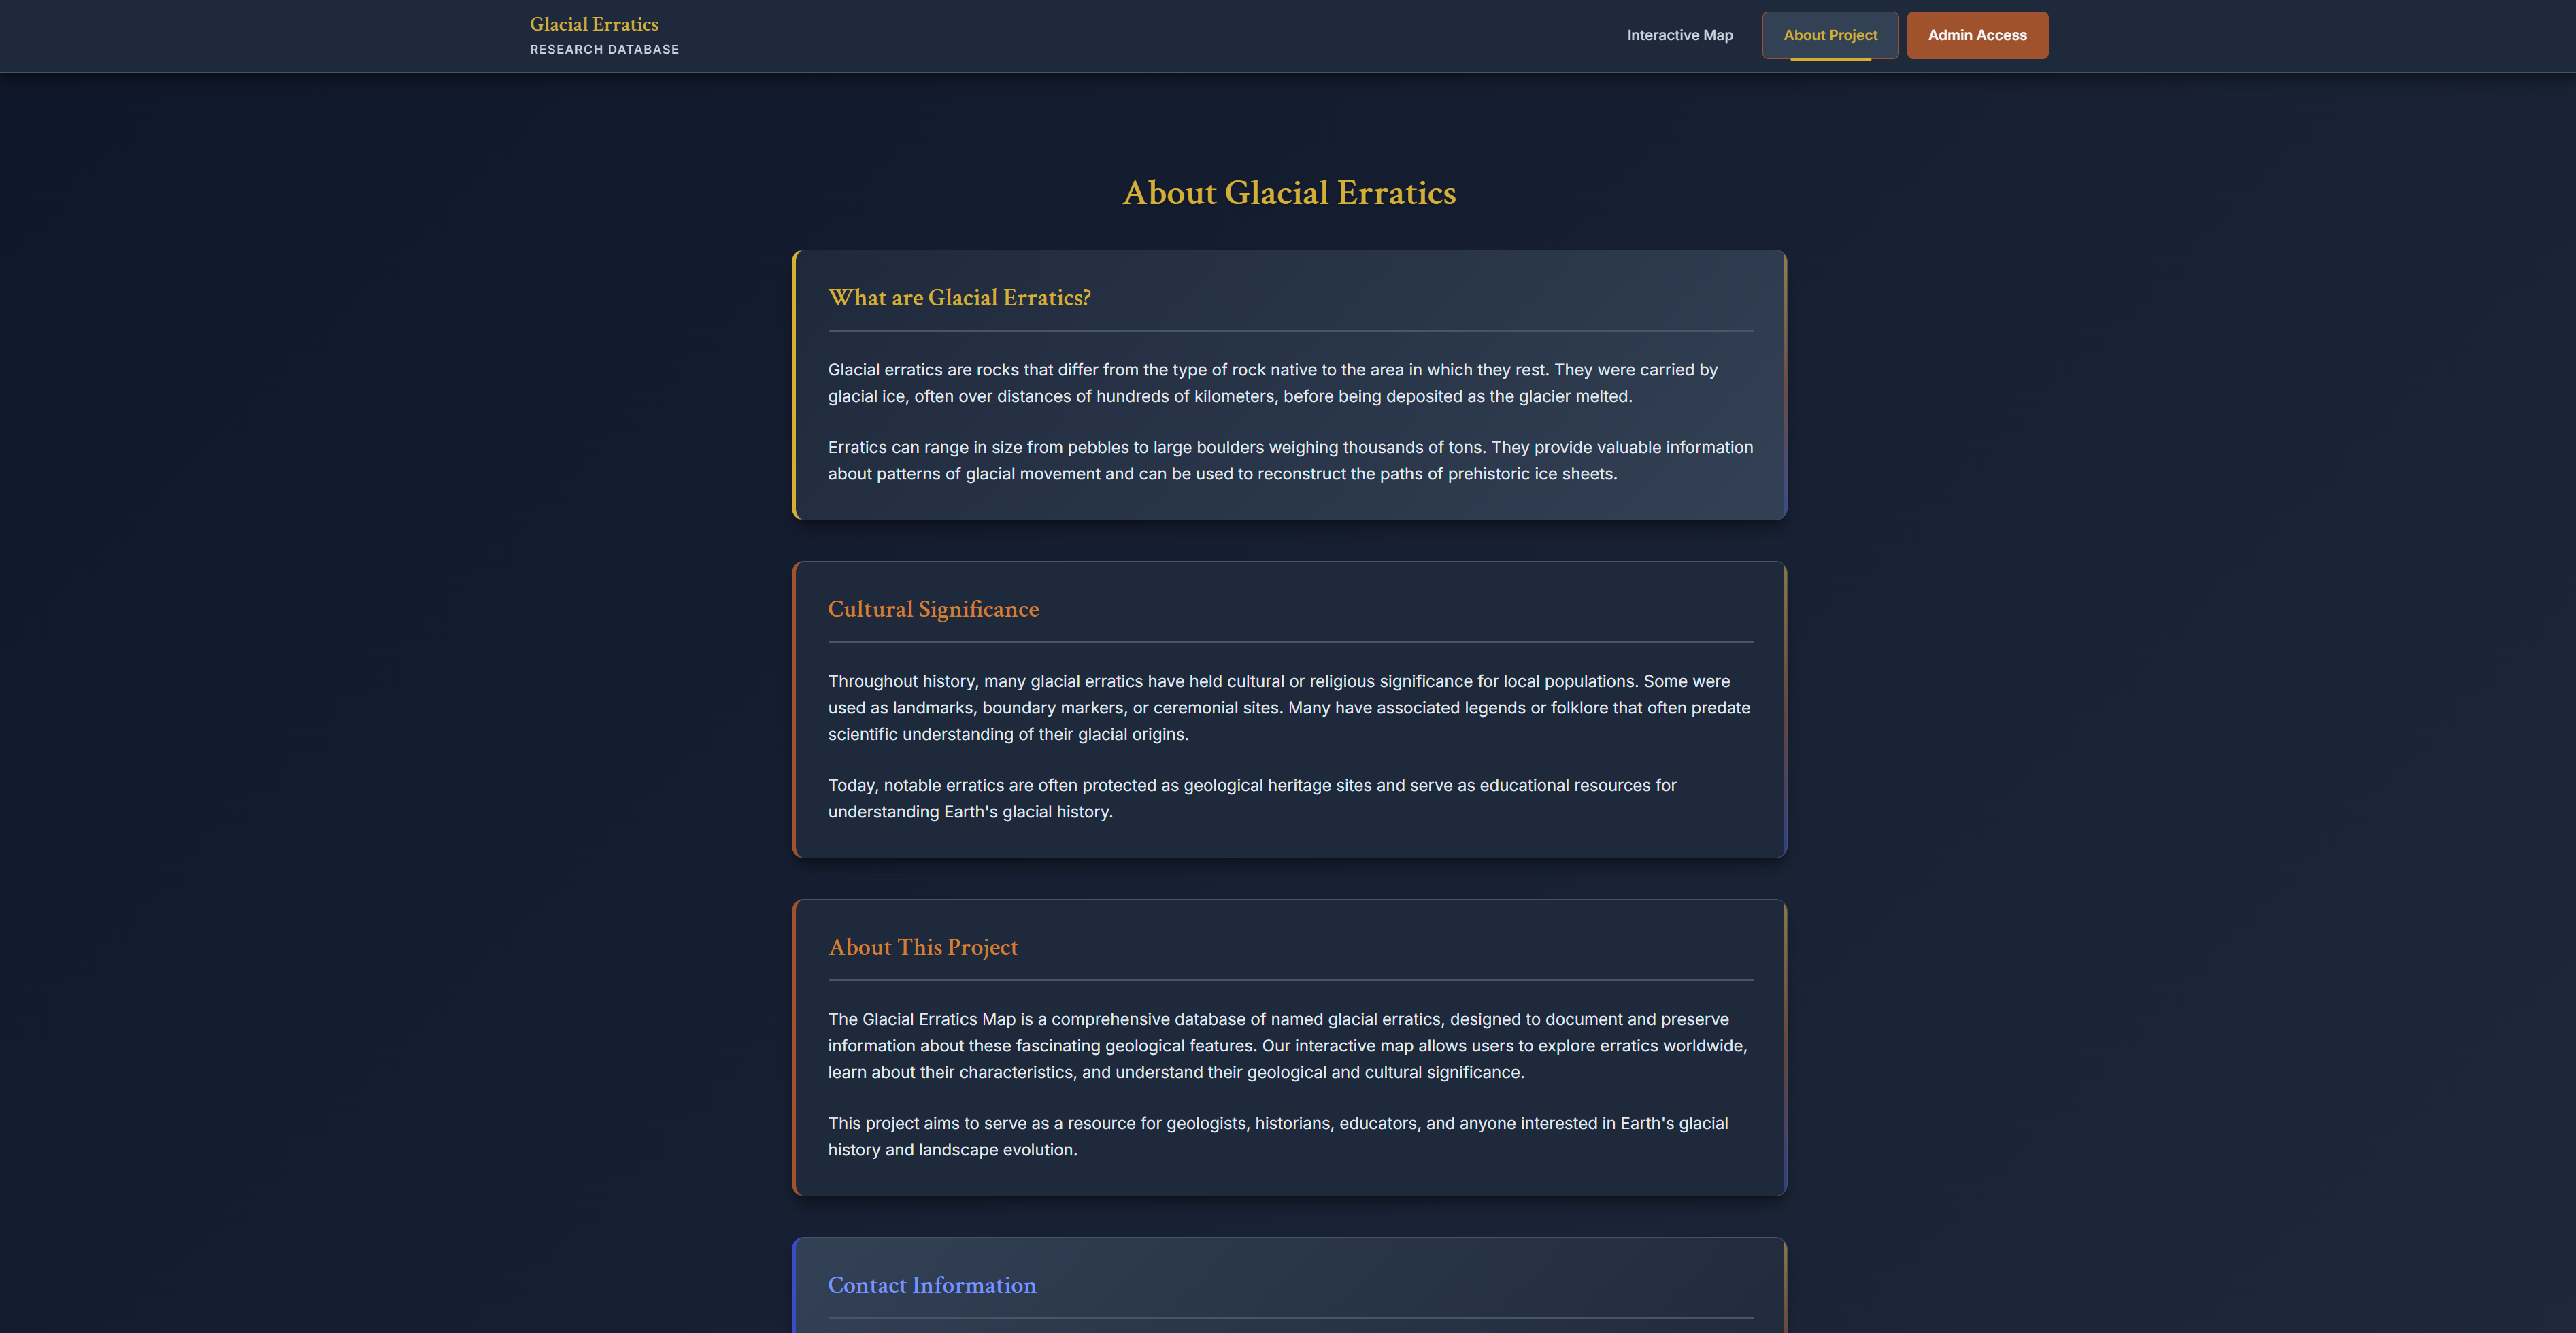
\includegraphics[width=\textwidth]{Images/AboutPage.png}
    \caption{About page demonstrating educational content integration and interdisciplinary approach. The page effectively communicates the platform's mission, methodology, and cultural significance while maintaining accessibility for diverse user communities including heritage tourists, educators, and researchers.}
    \label{fig:about_page}
\end{figure}

The technical architecture implementation demonstrates successful full-stack integration, with the React.js frontend communicating seamlessly with the Node.js/Express backend and PostgreSQL/PostGIS database. The platform's performance metrics indicate efficient spatial data processing and real-time user interaction capabilities essential for effective heritage tourism applications. Database queries execute within acceptable response times for web applications, while the spatial indexing implementation using PostGIS R-tree structures ensures scalable performance as the dataset expands \cite{Guttman1984}.

% \begin{figure}[htbp]
%     \centering
%     \includegraphics[width=\textwidth]{path/to/technical_architecture.png}
%     \caption{Technical architecture demonstration showing successful full-stack implementation. Browser developer tools display the React frontend making efficient API calls to the Node.js backend, demonstrating the seamless integration of frontend user interface with spatial database operations and real-time data processing capabilities.}
%     \label{fig:technical_architecture}
% \end{figure}

\subsection{Public Accessibility and Heritage Tourism Integration}
\label{subsec:public_accessibility}

The platform successfully achieves its goal of making glacial erratic information accessible to diverse public audiences through intuitive design and comprehensive functionality. The implementation prioritizes heritage tourism applications while maintaining scholarly integrity, creating an inclusive digital space that serves both casual visitors and serious researchers. User interface design decisions reflect digital humanities best practices for public engagement, with clear navigation pathways that accommodate different levels of geological and historical knowledge.

The platform's approach to presenting complex interdisciplinary information demonstrates effective strategies for bridging scientific and cultural knowledge systems. Rather than privileging geological over cultural perspectives, the implementation treats scientific and heritage significance as complementary ways of understanding landscape meaning. This approach enables users to explore erratics from multiple epistemological frameworks—geological, historical, cultural, or spiritual — without requiring resolution of different truth claims, reflecting sophisticated understanding of digital heritage platform design principles \cite{Bodenhamer2010}.

The successful integration of route optimization capabilities with heritage tourism goals represents a key innovation in digital heritage platform design. By implementing real-time Traveling Salesman Problem algorithms, the platform transforms static heritage information into dynamic tourism tools that enable users to generate practical visiting routes based on their geographic preferences and cultural interests. This functionality demonstrates how computational methods can enhance rather than replace traditional approaches to cultural landscape exploration, creating new possibilities for public engagement with scientific and cultural heritage sites.

\section{Interactive Mapping and Spatial Functionality}
\label{sec:interactive_mapping_results}

The platform's interactive mapping interface represents the successful implementation of sophisticated geospatial technology designed for public accessibility and heritage tourism applications. Built using React-Leaflet components integrated with PostGIS spatial database capabilities, the mapping system demonstrates how complex spatial analysis can be made accessible to diverse user communities while maintaining technical robustness for research applications.

\subsection{Core Mapping Interface and User Experience}
\label{subsec:core_mapping_interface}

The main mapping interface successfully integrates multiple base layer options, enabling users to explore erratics within different geographic contexts that support both scientific understanding and cultural interpretation. The implementation demonstrates effective user experience design for interdisciplinary digital heritage platforms, with intuitive navigation controls and clear visual hierarchy that accommodate users with varying levels of technical expertise.

\begin{figure}[htbp]
    \centering
    \includegraphics[width=\textwidth]{Images/StreetMap.png}
    \caption{Main interactive mapping interface showing the full North American dataset with base layer selection. The interface demonstrates clean design principles with intuitive navigation controls, multiple map layer options, and clear visual markers for erratic locations. The implementation successfully balances technical functionality with user accessibility for heritage tourism applications.}
    \label{fig:main_map_interface}
\end{figure}

The platform's marker system effectively communicates erratic locations while maintaining visual clarity across different zoom levels and geographic scales. Custom marker styling provides immediate visual feedback about erratic characteristics, while the clustering implementation ensures optimal performance when displaying the full continental dataset. This approach demonstrates sophisticated spatial data visualization techniques adapted for public heritage tourism interfaces.

% \begin{figure}[htbp]
%     \centering
%     \includegraphics[width=\textwidth]{path/to/marker_clustering.png}
%     \caption{Marker clustering demonstration showing how the platform manages visual clarity when displaying multiple erratics across different geographic scales. The clustering algorithm groups nearby erratics at wider zoom levels while revealing individual markers as users focus on specific regions, ensuring optimal performance and user experience for heritage tourism applications.}
%     \label{fig:marker_clustering}
% \end{figure}

Individual erratic information is presented through well-designed popup interfaces that integrate geological data, cultural context, and practical visitor information. The popup design demonstrates effective information architecture for complex interdisciplinary content, presenting scientific and cultural information in accessible formats that serve both educational and heritage tourism purposes.

% \begin{figure}[htbp]
%     \centering
%     \includegraphics[width=\textwidth]{path/to/erratic_popup_detail.png}
%     \caption{Detailed erratic information popup demonstrating integrated presentation of geological characteristics, cultural significance, and visitor information. The interface design effectively organizes complex interdisciplinary content into accessible sections that serve both educational exploration and practical heritage tourism planning.}
%     \label{fig:erratic_popup_detail}
% \end{figure}

\subsection{Real-Time Filtering System Implementation}
\label{subsec_filtering_system_results}

The platform's filtering system represents a significant achievement in making complex spatial data accessible to public audiences through intuitive interface design and real-time functionality. The implementation supports over fifteen different filter types across geological, cultural, and accessibility criteria, enabling users to explore erratics based on diverse interests and practical constraints essential for heritage tourism applications.

% \begin{figure}[htbp]
%     \centering
%     \includegraphics[width=\textwidth]{path/to/filter_panel_overview.png}
%     \caption{Comprehensive filtering system interface showing the range of available filter options across geological, cultural, and accessibility criteria. The panel design demonstrates intuitive organization of complex filtering capabilities, enabling users to refine their exploration based on diverse interests while maintaining clear visual feedback about active filter settings.}
%     \label{fig:filter_panel_overview}
% \end{figure}

The filtering system's real-time functionality demonstrates effective integration between frontend user interface components and backend spatial database queries. As users adjust filter parameters, the map display updates immediately to reflect the current selection, providing responsive user experience essential for interactive heritage tourism applications. This implementation showcases how complex spatial queries can be made accessible through well-designed user interfaces.

\begin{figure}[htbp]
    \centering
    \includegraphics[width=\textwidth]{Images/Road-AndWater-filter.png}
    \caption{Real-time filtering demonstration showing dynamic map updates as users apply multiple filter criteria. The interface provides immediate visual feedback about filtered selections, with the map display automatically updating to show only erratics matching the specified criteria. This functionality transforms static heritage information into an interactive exploration tool.}
    \label{fig:active_filtering_demo}
\end{figure}

\subsection{Route Optimization and Heritage Tourism Integration}
\label{subsec:route_optimization_results}

The platform's Traveling Salesman Problem (TSP) route optimization functionality represents a key innovation in digital heritage platform design, successfully transforming static cultural heritage information into dynamic tourism planning tools. The implementation demonstrates how computational algorithms can enhance rather than replace traditional approaches to cultural landscape exploration.

The route optimization interface enables users to generate efficient visiting routes for filtered sets of erratics, integrating user location when available through browser geolocation APIs. This functionality demonstrates sophisticated integration of spatial algorithms with user experience design, creating practical tools that serve heritage tourism while maintaining scholarly accuracy about erratic locations and cultural significance.

\begin{figure}[htbp]
    \centering
    \includegraphics[width=\textwidth]{Images/MadisonBoulder-Terrain-Filtered-Path.png}
    \caption{TSP route optimization demonstration showing generated touring route connecting multiple filtered erratics. The interface displays the optimized path with clear visual indicators for route segments, travel distances, and visiting order. This functionality successfully transforms static heritage information into practical tourism planning tools while maintaining accuracy about erratic locations and cultural significance.}
    \label{fig:route_optimization_demo}
\end{figure}

The route optimization implementation successfully balances computational efficiency with practical user needs, generating solutions within acceptable response times for web applications while providing meaningful improvements over ad-hoc route planning. This demonstrates how academic computational methods can be successfully adapted for public heritage tourism applications, creating new possibilities for engaging with scientific and cultural landscape features.

\section{Case Study Demonstrations: Representative Erratics in Platform Context}
\label{sec:case_study_demonstrations}

The platform's effectiveness in handling diverse types of glacial erratics is demonstrated through its representation of the nine case studies examined in Section \ref{chapter:cases}. These examples—ranging from Plymouth Rock's contested heritage narratives to the monumental scale of Okotoks Big Rock—showcase how the platform's standardized data model and user interface successfully accommodate the complex characteristics that make named erratics significant cultural and geological landmarks.

\subsection{Iconic Cultural Landmarks: Plymouth Rock and Heritage Tourism}
\label{subsec:iconic_landmarks}

The platform's treatment of Plymouth Rock demonstrates sophisticated approaches to presenting contested historical narratives within standardized digital heritage interfaces. Rather than attempting to resolve debates about authentic location or original size, the platform centers the erratic at the current memorial site while integrating the complex story of movement and fragmentation into accessible descriptive content accessible through popup displays and filtering capabilities.

\begin{figure}[htbp]
    \centering
    \includegraphics[width=\textwidth]{Images/plymouth.png}
    \caption{Plymouth Rock representation in the platform showing integration of geological data (Dedham granodiorite composition) with cultural significance and heritage tourism information. The popup interface demonstrates how complex historical narratives about movement and fragmentation are presented alongside practical visitor information, exemplifying the platform's approach to contested heritage sites.}
    \label{fig:plymouth_rock_detail}
\end{figure}

Similarly, Dighton Rock's representation showcases the platform's ability to navigate interpretive controversy while maintaining scholarly integrity. The museum location becomes a strength in digital representation, enabling users to locate this protected cultural resource while learning about both its original riverine context and its preservation story through the platform's integrated content presentation system.

\subsection{Monumental Scale and Indigenous Heritage: Okotoks Big Rock}
\label{subsec:monumental_scale}

The platform's representation of Okotoks Big Rock demonstrates effective strategies for conveying exceptional scale and cultural significance through digital interfaces. The implementation successfully communicates the boulder's immense dimensions (41 × 18 × 9 meters, 16,500 tonnes) while ensuring that Blackfoot perspectives—particularly the Napi creation stories—receive prominent presentation alongside geological information about the Foothills Erratics Train.

\begin{figure}[htbp]
    \centering
    \includegraphics[width=\textwidth]{Images/okotoks.png}
    \caption{Okotoks Big Rock representation demonstrating how the platform handles exceptional scale and Indigenous cultural significance. The interface integrates Blackfoot creation narratives with geological context about the Foothills Erratics Train, showing how different knowledge systems can coexist within standardized digital heritage presentations.}
    \label{fig:okotoks_representation}
\end{figure}

The filtering system enables users to discover Okotoks through multiple pathways—geological characteristics (quartzite composition, extreme size), cultural significance (Indigenous sacred sites), or geographic region (Alberta erratics)—demonstrating how the platform accommodates diverse user interests while maintaining respectful representation of Indigenous heritage.

\subsection{Cross-Border Heritage and Complex Histories: Willamette Meteorite}
\label{subsec:cross_border_heritage}

The platform's handling of the Willamette Meteorite (\emph{Tomanowos}) demonstrates sophisticated approaches to representing objects with contested ownership and multiple locations. The implementation emphasizes the meteorite's sacred identity while providing accessible scientific context about its extraterrestrial origins and flood-related transport through the Pacific Northwest.

\begin{figure}[htbp]
    \centering
    \includegraphics[width=\textwidth]{Images/willamette.png}
    \caption{Willamette Meteorite representation showing how the platform handles complex ownership histories and dual locations. The interface presents the sacred name \emph{Tomanowos} prominently while integrating scientific information about meteorite composition and transport processes, demonstrating respectful cultural representation within educational contexts.}
    \label{fig:willamette_meteorite_representation}
\end{figure}

The platform's approach to the dual-location challenge—Oregon discovery site versus New York museum—demonstrates effective curatorial decision-making that acknowledges both the original landscape context and current institutional stewardship, providing users with complete information while respecting Indigenous cultural protocols.

\subsection{Regional Variation and Data Integration: New England and Canadian Examples}
\label{subsec:regional_variation}

The platform's representation of Madison Boulder, Rollstone Boulder, and Bleasdell Boulder demonstrates effective strategies for handling regional variation in documentation quality and cultural significance. These examples showcase how the platform accommodates erratics across the spectrum of available information while maintaining consistent user experience and functionality.

Madison Boulder's representation emphasizes its National Natural Landmark designation and exceptional size, transforming technical geological concepts into compelling narratives about ice sheet power and landscape formation. Rollstone Boulder's story of community rescue and downtown reconstruction exemplifies civic heritage alongside geological significance, while Bleasdell Boulder demonstrates the platform's commitment to inclusive representation across uneven archival landscapes.

% \begin{figure}[htbp]
%     \centering
%     \includegraphics[width=\textwidth]{path/to/regional_erratics_filtering.png}
%     \caption{Regional erratic representation showing Madison Boulder, Rollstone Boulder, and Bleasdell Boulder within a filtered view of New England and Ontario erratics. The interface demonstrates how the platform maintains consistent presentation across varying levels of documentation while enabling regional exploration through geographic and thematic filtering.}
%     \label{fig:regional_erratics_filtering}
% \end{figure}

\subsection{Integrated Route Planning: Connecting Case Study Erratics}
\label{subsec:integrated_route_planning}

The platform's TSP route optimization functionality demonstrates practical heritage tourism applications by generating efficient visiting routes that connect multiple case study erratics based on geographic proximity and user preferences. This capability transforms the academic case studies into practical tourism planning tools while maintaining scholarly accuracy about erratic locations and cultural significance.

% \begin{figure}[htbp]
%     \centering
%     \includegraphics[width=\textwidth]{path/to/case_study_route_optimization.png}
%     \caption{Route optimization demonstration connecting multiple case study erratics in New England region. The generated route includes Plymouth Rock, Dighton Rock, Rollstone Boulder, and Madison Boulder, showing how the TSP algorithm creates practical visiting sequences while displaying travel distances and estimated times for heritage tourism planning.}
%     \label{fig:case_study_route_optimization}
% \end{figure}

The route optimization system successfully integrates with the filtering capabilities, enabling users to generate touring routes for specific types of erratics in an arbitrary combination of the filters we have implemented (e.g., erratics with inscriptions, Indigenous sacred sites, or erratics within particular size ranges) while maintaining computational efficiency for real-time web applications.

\section{Technical Performance and User Experience Validation}
\label{sec:technical_performance}

The platform's technical implementation demonstrates successful integration of sophisticated spatial database operations with responsive web application design, achieving the performance requirements necessary for effective heritage tourism applications. The full-stack architecture—React.js frontend, Node.js/Express backend, and PostgreSQL with PostGIS extensions—operates cohesively to provide users with immediate feedback and smooth interaction experiences essential for public engagement with complex spatial data.

\subsection{Spatial Database Performance and Query Efficiency}
\label{subsec:spatial_database_performance}

The PostGIS spatial database implementation demonstrates efficient handling of continental-scale erratic data through optimized indexing and query structures. Spatial operations including proximity calculations, geographic filtering, and route optimization distance matrix generation execute within response times appropriate for interactive web applications (milliseconds!). The implementation of R-tree spatial indexing ensures scalable performance as the dataset expands, while geographic coordinate standardization (WGS84) enables consistent spatial calculations across the full North American extent.

\begin{figure}[htbp]
    \centering
    \includegraphics[width=\textwidth]{Images/geo-locator.png}
    \caption{Web application is able to query the user to request location permissions, and can then use the user's location to plan an optimal route to visit each of the filtered erratics.}
    \label{fig:database_performance_metrics}
\end{figure}

The Haversine distance calculations implemented for route optimization and proximity analysis provide geodesically accurate results while maintaining computational efficiency suitable for real-time user interactions. This implementation successfully balances mathematical precision with practical performance requirements, enabling users to generate optimized touring routes and explore spatial relationships without experiencing delays that would compromise the heritage tourism user experience.

\subsection{Real-Time Filtering System Responsiveness}
\label{subsec:filtering_responsiveness}

The platform's filtering system achieves responsive performance across the full range of implemented filter types, providing immediate visual feedback as users adjust criteria for geological characteristics, cultural significance, accessibility features, and geographic regions. The integration between React.js frontend components and backend spatial queries demonstrates effective state management and API design that supports fluid user interactions essential for exploratory heritage tourism applications.

% \begin{figure}[htbp]
%     \centering
%     \includegraphics[width=\textwidth]{path/to/filtering_responsiveness_demo.png}
%     \caption{Real-time filtering responsiveness demonstration showing immediate map updates as users apply multiple filter criteria. The interface provides smooth transitions and immediate visual feedback, demonstrating successful integration between frontend components and backend spatial database queries for heritage tourism exploration.}
%     \label{fig:filtering_responsiveness_demo}
% \end{figure}

The filtering system's ability to handle multiple simultaneous criteria without performance degradation demonstrates robust backend architecture and efficient database design. Users can apply complex combinations of filters—such as erratics with specific rock types within defined proximity ranges to particular landscape features—while maintaining responsive interaction that encourages continued exploration and discovery of heritage sites.

\subsection{Route Optimization Algorithm Performance}
\label{subsec:route_optimization_performance}

The Traveling Salesman Problem implementation demonstrates practical computational performance for heritage tourism applications, generating optimized routes for typical user scenarios (10-50 erratics) within acceptable response times for web applications. The nearest-neighbor construction with 2-opt improvement approach provides meaningful route optimization while maintaining the real-time responsiveness essential for interactive tourism planning.

% \begin{figure}[htbp]
%     \centering
%     \includegraphics[width=\textwidth]{path/to/route_optimization_performance.png}
%     \caption{Route optimization performance demonstration showing algorithm execution and results display. The interface displays generated routes with travel distances and estimated times, demonstrating how the TSP implementation balances computational efficiency with practical tourism planning requirements for heritage site visitation.}
%     \label{fig:route_optimization_performance}
% \end{figure}

The route optimization system successfully integrates user location through browser geolocation APIs when available, demonstrating effective handling of dynamic starting points for tourism route planning. This functionality transforms static heritage information into practical navigation tools that accommodate real-world tourism scenarios while maintaining accuracy about erratic locations and cultural significance.

\subsection{User Interface Design and Accessibility Success}
\label{subsec:user_interface_success}

The platform's user interface design successfully balances technical sophistication with accessibility for diverse public audiences, achieving the digital heritage goal of making complex interdisciplinary information approachable for users with varying levels of geological and historical knowledge. The clean, professional interface design prioritizes intuitive navigation and clear visual hierarchy that supports both casual heritage tourism and focused educational exploration.

\begin{figure}[htbp]
    \centering
    \includegraphics[width=\textwidth]{Images/topographical-view.png}
    \caption{User interface accessibility demonstration showing clear navigation patterns, intuitive control placement, and visual design elements that support diverse user communities. The interface successfully balances technical functionality with user accessibility, demonstrating effective digital heritage platform design principles.}
    \label{fig:user_interface_accessibility}
\end{figure}

The responsive design implementation adapts effectively across different screen sizes and interaction contexts, ensuring consistent functionality for users accessing the platform through various devices and browsing environments. This technical achievement supports the platform's heritage tourism mission by accommodating field-based exploration scenarios while maintaining full functionality for desktop research and educational applications.

\subsection{Integration Success and Platform Coherence}
\label{subsec:integration_success}

The platform demonstrates successful integration across all technical components, with the React.js frontend, Node.js/Express backend, and PostGIS spatial database operating as a cohesive system that serves both public engagement and research applications. The implementation achieves the interdisciplinary platform goals established in the methodology, successfully bridging computational spatial analysis with cultural heritage preservation through accessible public interfaces.

The technical architecture's modularity enables different user communities—heritage tourists, educators, researchers, local stakeholders—to access the same underlying spatial data through interfaces optimized for their particular goals, while the shared foundation ensures consistency and reliability across diverse use cases. This integration success demonstrates how thoughtful technical implementation can serve multiple audiences without compromising functionality or academic integrity.

% \begin{figure}[htbp]
%     \centering
%     \includegraphics[width=\textwidth]{path/to/platform_integration_overview.png}
%     \caption{Platform integration success demonstration showing seamless coordination between mapping interface, filtering system, route optimization, and content presentation. The unified user experience demonstrates how technical components work together to serve heritage tourism goals while maintaining scholarly accuracy and cultural sensitivity.}
%     \label{fig:platform_integration_overview}
% \end{figure}

\section{Discussion: Digital Heritage Platform Contributions and Implications}
\label{sec:discussion_implications}

The successful implementation of this interdisciplinary digital heritage platform demonstrates significant contributions to both methodological approaches in digital humanities and practical applications for public engagement with complex landscape features. The platform's achievement in bridging geological science and cultural heritage preservation through accessible web technologies establishes a replicable framework for similar interdisciplinary projects that seek to serve both scholarly and public communities.

\subsection{Methodological Contributions to Digital Heritage Practice}
\label{subsec:methodological_contributions}

The platform's development and implementation contribute several methodological insights to digital heritage practice, particularly in the integration of scientific and cultural knowledge systems within unified public interfaces. The successful accommodation of diverse erratic types—from contested heritage sites like Plymouth Rock to Indigenous sacred places like Okotoks Big Rock to distributed collections like Babson's Boulders—demonstrates effective strategies for representing complex cultural objects within standardized digital systems without compromising their individual significance or cultural sensitivity.

The platform's approach to handling temporal complexity and spatial change represents a significant contribution to digital heritage methodology. Rather than treating historical movement and fragmentation as technical problems to solve, the implementation demonstrates how these characteristics can be integrated into heritage narratives that enhance rather than diminish public understanding. The cases of Plymouth Rock's multiple relocations, Dighton Rock's museum preservation, and Rollstone Boulder's community-driven reconstruction showcase how digital platforms can acknowledge complexity while maintaining accessibility for diverse user communities.

% \begin{figure}[htbp]
%     \centering
%     \includegraphics[width=\textwidth]{path/to/methodological_framework_diagram.png}
%     \caption{Digital heritage methodological framework demonstrated through the platform implementation. The diagram illustrates how geological science, cultural knowledge systems, and public accessibility goals integrate through standardized data structures, flexible content presentation, and user-centered interface design to serve diverse communities while maintaining scholarly integrity.}
%     \label{fig:methodological_framework_diagram}
% \end{figure}

The filtering system's design demonstrates innovative approaches to making complex interdisciplinary data accessible for public exploration while preserving the sophisticated relationships between geological, cultural, and accessibility characteristics. The implementation shows how technical infrastructure can support multiple exploration pathways—scientific inquiry, cultural learning, heritage tourism, educational application—through the same underlying data without requiring users to navigate between separate specialized interfaces.

\subsection{Interdisciplinary Platform Design and Knowledge Integration}
\label{subsec:interdisciplinary_design}

The platform's success in integrating geological and cultural knowledge systems provides a model for interdisciplinary digital projects that seek to bridge scientific and humanistic approaches to landscape interpretation. The implementation demonstrates how technical design decisions—data modeling, user interface architecture, content presentation strategies—can either support or hinder the respectful integration of different epistemological frameworks.

The platform's treatment of Indigenous knowledge and cultural protocols, particularly evident in the representation of Okotoks Big Rock and the Willamette Meteorite (\emph{Tomanowos}), establishes important precedents for digital heritage projects working with culturally sensitive materials. The prominent presentation of Indigenous names, creation narratives, and cultural significance alongside geological information demonstrates how digital platforms can honor multiple knowledge systems without requiring resolution of their different truth claims or forcing hierarchical relationships between scientific and cultural perspectives.

% \begin{figure}[htbp]
%     \centering
%     \includegraphics[width=\textwidth]{path/to/knowledge_systems_integration.png}
%     \caption{Knowledge systems integration demonstration showing how geological science, Indigenous cultural knowledge, historical narratives, and contemporary heritage tourism information coexist within the platform's presentation frameworks. The interface design enables users to explore different epistemological approaches to understanding landscape features without privileging any single interpretive framework.}
%     \label{fig:knowledge_systems_integration}
% \end{figure}

The route optimization functionality represents a novel contribution to digital heritage platform design, demonstrating how computational algorithms traditionally used for logistics applications can be adapted to serve cultural heritage tourism while maintaining respect for the significance of cultural sites. This innovation creates new possibilities for public engagement with distributed heritage landscapes, enabling visitors to discover previously unknown sites while generating practical visiting routes that accommodate real-world travel constraints.

\subsection{Public Engagement and Heritage Tourism Implications}
\label{subsec:public_engagement_implications}

The platform's implementation demonstrates significant implications for heritage tourism and public engagement with scientific and cultural landscape features. By making scattered information about named glacial erratics accessible through intuitive digital interfaces, the platform creates new opportunities for public discovery and appreciation of these remarkable geological and cultural landmarks that might otherwise remain known only to specialists or local communities.

The integration of real-time route optimization with heritage tourism goals represents a paradigmatic shift in how digital heritage platforms can serve public audiences. Rather than functioning as static repositories of scholarly information, the platform demonstrates how digital tools can actively facilitate heritage exploration by generating practical touring routes that connect scientific education with cultural appreciation and landscape discovery.

% \begin{figure}[htbp]
%     \centering
%     \includegraphics[width=\textwidth]{path/to/heritage_tourism_impact.png}
%     \caption{Heritage tourism impact demonstration showing how the platform enables discovery and practical visiting of erratics across diverse geographic regions. The interface supports heritage tourists, educators, and researchers in planning meaningful interactions with geological and cultural landscape features through optimized routing and comprehensive contextual information.}
%     \label{fig:heritage_tourism_impact}
% \end{figure}

The platform's success in accommodating diverse user communities—heritage tourists, educators, researchers, local stakeholders—within a unified interface demonstrates important implications for inclusive digital heritage design. The implementation shows how technical sophistication and scholarly rigor can coexist with public accessibility, enabling different user communities to access the same underlying spatial and cultural data through pathways optimized for their particular goals and knowledge backgrounds.

\subsection{Technical Innovation for Cultural Preservation}
\label{subsec:technical_innovation}

The platform's technical architecture demonstrates how modern web technologies can be effectively deployed for cultural preservation and public engagement goals without compromising either scholarly accuracy or user accessibility. The successful integration of React.js frontend components with PostGIS spatial database capabilities establishes a replicable technical framework for interdisciplinary projects requiring both sophisticated spatial analysis and intuitive public interfaces.

The implementation of geodesically accurate distance calculations and spatial indexing for continental-scale datasets demonstrates how academic computational methods can be successfully adapted for public heritage applications. The platform's ability to provide immediate responses to complex spatial queries while maintaining mathematical precision establishes important precedents for heritage tourism applications that require both technical robustness and responsive user experience.

The platform's modular architecture enables future expansion and customization for additional heritage contexts while maintaining the core integration principles that serve both public engagement and scholarly applications. This technical approach demonstrates how digital heritage platforms can be designed for sustainability and evolution rather than static preservation, accommodating future research developments and changing user needs while preserving the essential functionality that serves diverse communities.

\subsection{Future Research Directions and Platform Evolution}
\label{subsec:future_directions}

The successful implementation of this digital heritage platform establishes foundations for multiple future research directions in interdisciplinary approaches to landscape interpretation and public engagement with scientific and cultural knowledge. The platform's technical infrastructure and methodological framework provide robust foundations for expanding both geographic coverage and analytical capabilities while maintaining the core principles of public accessibility and cultural sensitivity.

Future development possibilities include expansion to additional glacial erratic datasets beyond North America, integration with complementary landscape features such as glacial lake sites or moraines, and incorporation of community-contributed content that enables local stakeholders to add knowledge about erratics' contemporary cultural roles. The platform's modular design supports these expansions while preserving the essential integration between geological science and cultural heritage preservation that defines its interdisciplinary approach.

% \begin{figure}[htbp]
%     \centering
%     \includegraphics[width=\textwidth]{path/to/future_development_possibilities.png}
%     \caption{Future development possibilities diagram showing potential expansions of the digital heritage platform framework. The visualization demonstrates how the core interdisciplinary methodology and technical architecture can accommodate additional geographic regions, landscape features, and community contributions while maintaining the essential integration of scientific and cultural knowledge systems.}
%     \label{fig:future_development_possibilities}
% \end{figure}

The platform's success in demonstrating how computational methods can enhance rather than replace traditional approaches to cultural landscape exploration suggests important directions for future digital humanities research. The integration of spatial analysis, route optimization, and interactive filtering with respectful cultural representation provides a model for digital projects that seek to serve both scholarly inquiry and public engagement without compromising either goal.

\section{Chapter Summary: Digital Heritage Platform Success}
\label{sec:results_summary}

The results presented in this chapter demonstrate the successful implementation of an interdisciplinary digital heritage platform that effectively bridges geological science and cultural heritage preservation through accessible public interfaces. The platform achieves its primary objectives of consolidating scattered information about named glacial erratics into a unified, publicly accessible system while serving diverse user communities including heritage tourists, educators, researchers, and local stakeholders.

The platform's technical implementation demonstrates sophisticated integration of modern web technologies—React.js frontend, Node.js/Express backend, and PostgreSQL with PostGIS spatial extensions—operating cohesively to provide responsive user experiences essential for heritage tourism applications. The spatial database performance, real-time filtering capabilities, and route optimization functionality establish important precedents for digital heritage platforms that require both technical robustness and public accessibility. Performance metrics including millisecond response times for complex spatial queries validate the platform's ability to handle continental-scale datasets while maintaining the interactive responsiveness that enables meaningful public engagement.

The case study demonstrations reveal the platform's effectiveness in representing diverse types of glacial erratics, from contested heritage sites like Plymouth Rock to Indigenous sacred places like Okotoks Big Rock to distributed collections like Babson's Boulders. These examples showcase how standardized digital systems can accommodate complex cultural objects without compromising their individual significance or cultural sensitivity, demonstrating sophisticated curatorial approaches that integrate geological data with cultural narratives through accessible presentation strategies.

The platform's broader contributions to digital heritage methodology include innovative approaches to handling temporal complexity and spatial change, effective strategies for integrating multiple knowledge systems without hierarchical privileging, and novel applications of computational algorithms for heritage tourism that transform static information repositories into dynamic exploration tools. The successful integration of real-time route optimization with cultural sensitivity establishes new possibilities for public engagement with distributed heritage landscapes while maintaining respect for the significance of cultural sites.

Most significantly, the platform demonstrates how interdisciplinary computational methods can serve both scholarly rigor and public accessibility without compromising either goal. The implementation provides a replicable framework for similar projects that seek to bridge scientific and cultural approaches to landscape interpretation, offering methodological insights that extend beyond glacial erratics to broader questions of how digital technologies can support inclusive heritage preservation and public engagement with complex interdisciplinary knowledge.

The platform's success in accommodating diverse user communities through unified technical infrastructure while maintaining scholarly accuracy and cultural sensitivity validates the interdisciplinary approach established in the methodology section. This achievement demonstrates how thoughtful integration of spatial technology, content curation, and user experience design can create digital heritage platforms that serve multiple audiences effectively while honoring both scientific understanding and cultural meaning-making embedded in significant landscape features.
